\begin{figure}
	\begin{minipage}[b]{.5\linewidth}
		\centering
		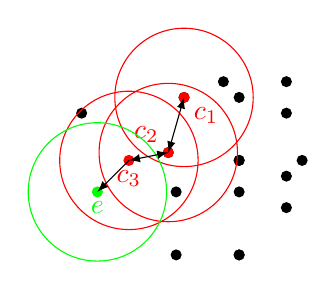
\begin{tikzpicture}
			\fill (-2,1.8) circle(2pt);
			\fill (-.9, 1.3) circle(2pt);
			\fill (-.8,.8) circle(2pt);
			\fill (-.8,0) circle(2pt);
			\fill (-.7,2) circle(2pt);
			\fill (-.2,2.2) circle(2pt);
			\fill (0,0) circle(2pt);
			\fill (0,1.2) circle(2pt);
			\fill (0,1.2) circle(2pt);
			\fill (0,0) circle(2pt);
			\fill (0,.8) circle(2pt);
			\fill (0,2) circle(2pt);
			\fill (.6,1) circle(2pt);
			\fill (.6,.6) circle(2pt);
			\fill (.6,1.8) circle(2pt);
			\fill (.6,2.2) circle(2pt);
			\fill (.8,1.2) circle(2pt);
			
			\fill[red] (-.7, 2) circle(2pt) node[anchor=north west]{$ c_1 $};
			\draw[red] (-.7, 2) circle(25pt);
			
			\fill[red] (-.9, 1.3) circle(2pt) node[anchor=south east]{$ c_2 $};
			\draw[red] (-.9, 1.3) circle(25pt);
			
			\fill[red] (-1.4,1.2) circle(2pt) node[anchor=north]{$ c_3 $};
			\draw[red] (-1.4,1.2) circle(25pt);
			
			\fill[green] (-1.8,.8) circle(2pt) node[anchor=north]{$ e $};
			\draw[green] (-1.8,.8) circle(25pt);
			
			\draw[latex-latex] (-.7, 2) -- (-.9, 1.3);
			\draw[latex-latex] (-.9, 1.3) -- (-1.4,1.2);
			\draw[-latex] (-1.4,1.2) -- (-1.8,.8);
		\end{tikzpicture}
		\subcaption{$ reach_{\varepsilon,\mu}(e, c_1) $} \label{fig:density-reachablity-reachability}
	\end{minipage}
	\begin{minipage}[b]{.5\linewidth}
		\centering
		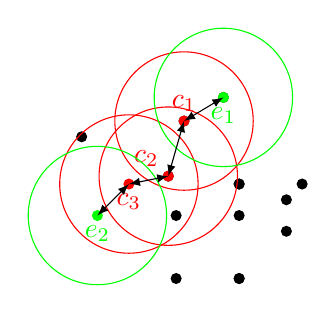
\begin{tikzpicture}
			\fill (-2,1.8) circle(2pt);
			\fill (-.9, 1.3) circle(2pt);
			\fill (-.8,.8) circle(2pt);
			\fill (-.8,0) circle(2pt);
			\fill (-.7,2) circle(2pt);
			\fill (-.2,2.3) circle(2pt);
			\fill (0,0) circle(2pt);
			\fill (0,1.2) circle(2pt);
			\fill (0,1.2) circle(2pt);
			\fill (0,0) circle(2pt);
			\fill (0,.8) circle(2pt);
			\fill (.6,1) circle(2pt);
			\fill (.6,.6) circle(2pt);
			\fill (.8,1.2) circle(2pt);
			
			\fill[red] (-.7, 2) circle(2pt) node[anchor=south]{$ c_1 $};
			\draw[red] (-.7, 2) circle(25pt);
			
			\fill[red] (-.9, 1.3) circle(2pt) node[anchor=south east]{$ c_2 $};
			\draw[red] (-.9, 1.3) circle(25pt);
			
			\fill[red] (-1.4,1.2) circle(2pt) node[anchor=north]{$ c_3 $};
			\draw[red] (-1.4,1.2) circle(25pt);
			
			\fill[green] (-1.8,.8) circle(2pt) node[anchor=north]{$ e_2 $};
			\draw[green] (-1.8,.8) circle(25pt);
			
			\fill[green] (-.2,2.3) circle(2pt) node[anchor=north]{$ e_1 $};
			\draw[green] (-.2,2.3) circle(25pt);
			
			\draw[latex-latex] (-.2,2.3) -- (-.7, 2);
			\draw[latex-latex] (-.7, 2) -- (-.9, 1.3);
			\draw[latex-latex] (-.9, 1.3) -- (-1.4,1.2);
			\draw[latex-latex] (-1.4,1.2) -- (-1.8,.8);
		\end{tikzpicture}
		\subcaption{$ connected_{\varepsilon,\mu}(e_1, e_2) $} \label{fig:density-reachablity-connection}
	\end{minipage}
	\caption{Relacje gęstościowej osiągalności \subref{fig:density-reachablity-reachability} oraz łączności \mbox{gęstościowej \subref{fig:density-reachablity-connection},} $ \mu = 3 $.}
\end{figure}